\section{Test vehicule description and failure signature}

This chapter focuses on the functionnal failure caused by an \gls{esd} of an integrated function.
The studied function is the primary supply of a complex automotive \gls{asic}.
This supply plays a critical role in the functionning of the entire product.
It is connected to the battery of the vehicle, and is the first block of the product to start.
It wakes up and powers all other functions inside the integrated circuit.

\begin{figure}[h]
  \centering
  
\includegraphics{src/4/figures/testchip_overview.pdf}
  \caption{Architecture of the studied functionnality}
  \label{testchip_overview}
\end{figure}

The primary supply processes the battery supply in a chained fashion (see Fig. \ref{testchip_overview}).
A first block (pre-regulator) clamps the battery voltage (that can reach up to 40V) to 9V, a more acceptable voltage for the silicium technology.
This clamped voltaged is then used to power up a bandgap reference.
Once properly started, this bandgap generates a 1.23 V voltage reference, stable accross a wide range of temperature, process variation and mismatchs.
The bandgap also outputs a 10uA current reference, stable in the same conditions.

After the bandgap, a \gls{ldo} regulator relies on the voltage reference to generate a stable 2.5V supply voltage, able to deliver and sustain up to 20mA.
This first regulator is connected externally to a 100nF decoupling capacitor to absorb peak currents and achieve stability.
This supply is used to supply most analog (digital ?) functions inside the integrated circuit.

A second regulator performs the same task, but starts with a delay compared to the first one.
It also ouputs a 2.5V supply, that powers digital logic inside the circuit.

In case of failure, the primary supply can cause the entire product to shut down.
Indeed, this entire system requires soft-start behavior to avoid generating harmful voltage spikes to powered functions.
This functionnality enforces the system to start on a \br{long} period of time, in the order of a hundred microseconds.

When the system is stressed with an \gls{esd}, voltages and currents are fluctuating inside the block.
Under certain conditions, and especially important stress levels, the block will detects some nodes going in undervoltage or overvoltage.
This will cause the block to go into safe or protected mode, where it will restart because the functionnality cannot be assured properly.
The direct consequence is that the block will require again a hundred microseconds to be again in normal operation mode.

This failure can in a first time be observed in simulation.
An \gls{ESD} is superimposed on the DC battery voltage.
This is the most likely entry point for a stress, because the \gls{IC} exposes a pin to the external workd and is usally connected to the battery via a long cable
To detect is a block reset happened, the voltage on the first voltage regulator is observed.
Fig. X shows the stress waveform on the input.

STRESS WAVEFORM INPUT

Fig. X shows a simulation where a small glitch can be observed on the regulated output, but without clear reset or soft-failure signature.
In this case, the block and the rest of the product is most likely not affected by the ESD.

WAVEFORM OUTPUT NO RESET

Fig. X shows a simulation where a clear reset hapened.
The output voltage is maintained by a 100nF capacitor.
However, it clearly goes down \br{after} the \gls{esd} and rises slowly afterward, a sign that the block went into full reset and restard.

WAVEFORM OUTPUT RESET

By going inside the \gls{IC}...

bandgap, voltage ref, current ref, etc

DISCUSSION AROUND INCREASE OF FAILURE LENGTH after each stage of the chain

\section{Bottom-up block failure modeling}
\label{sec:bottom-up-modeling}

\subsection{Block failure characterization and modeling method}
\label{sec:block-failure-cz}

% What is bottom up
The modelling method presented in this section focuses first on studying low-level cells of the circuit.
They are characterized individually, leading to the definition of a failure model for each cell.
In a second step, the individual models are linked together.
The connection between the models reproduce the connections between the cells in the actual circuit.
Finally, an electrical stimulus such as an electrostatic discharge is fed on the input of the first model.
It is applied on this model that produces an output signal.
In turn, this signal is used as stimulus for the second model in the chain which is using it as input.
The process is repeated until the last output, where the output signal represents the shape of the disturbance after going through the entire chain.

% Why bottom up
The main perk of this characterization method is the modularity, because each block is characterized independently of the others.
The model built for each cell is reusable, and once the characterization is done it does not need to be repeated unless modifications are brought to the circuit.
This method is called bottom-up because low-level functions components are characterized then assembled to model higher-level functions, rising from the bottom of the hierarchy to upper levels.

% Why modelling individual blocks
The motivation for modelling blocks individually is that a single block can be failing but the error can remain internal.
Complete function can continue to operate without changes.
In the other way around, not all blocks need to be failing in order to cause the complete function to fail as well.
It is important to determine which blocks may be in fault to be able to fix the problem.
This is why the characterization method presented here focuses on blocks and not complete functions.

% Models are not electrical but failure models
The goal of this method is to build a propagation model and not an electrical \gls{spice} model.
The models built here are not usable directly in standard simulations and does not produce strict waveforms on their ouputs.
Instead, they represent input and output waveforms by bounding boxes of a given amplitude and width.
The methodology is built on the hypothesis that simplified \gls{esd} waveforms could be sufficient to estimate the robustness of an integrated function.
This hypothesis is tested as detailed later in the document.

% Describe the changes
Several refinements of the modelling methods were applied to solve issues as they were encountered.
This chapter gives a logical history of those improvements in order to understand the starting phase and the modifications applied after.
Initially, Wunsch and Bell characterization \cite{wunsch-bell} is used to determine failure levels of individual cells when exposed to stresses of different width and amplitude.
A single failure criteria was preliminary established for each model.
It usually took the form of a voltage threshold applied on the output of a cell, above which a fault is recorded.
This treshold is set prior to the simulation, and there is no general rule for setting it.
The \gls{dc} specification of the output can be used directly, if it exists, or a sound value in regard of the design, or an arbitrary level.

% How is it done, core concept
The first part of the modelling method is the characterization of each block using the electrical setup of Fig. \ref{block_function_cz} in a \gls{spice} simulation environment.
This setup provides appropriate biasing to the block with V\textsubscript{DC} voltage source, in order to set the block function in operating conditions.
It also enables the injection of the characterization signal on the tested input with V\textsubscript{stress} transient voltage source.
The characterization pulses are rectangular waveforms similarly to the Wunsch and Bell technique.
Each simulation runs with a different pair of values for the \textbf{amplitude} and \textbf{duration} of the square signal.
On the other side of the cell under test, the output is monitored.
Prior to the simulation, a failure criteria consisting of a voltage threshold is set.
If the output waveform goes above this threshold, the simulation is tagged as \textit{fail}.
The threshold is chosen depending on multiple parameters such as the functionality of the block or its DC operating point.

\begin{figure}[!h]
  \centering
  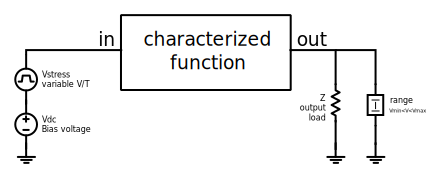
\includegraphics{src/4/figures/characterization_setup.pdf}
  \caption{Block characterization setup (supply input)}
  \label{block_function_cz}
\end{figure}

The results are summarized into table \ref{simulation-results}.
The simulations in red contain a fail, meaning that the output voltage crossed the failure threshold.

\begin{table}[!h]
\centering
\begin{tabular}{@{}lllll@{}}
\toprule
    & 1ns                          & 10ns                         & 100ns                        & 1\textmugreek{}s             \\ \midrule
15V & {\color[HTML]{FE0000} sim13} & {\color[HTML]{FE0000} sim23} & {\color[HTML]{FE0000} sim33} & {\color[HTML]{FE0000} sim43} \\
10V & {\color[HTML]{32CB00} sim12} & {\color[HTML]{FE0000} sim22} & {\color[HTML]{FE0000} sim32} & {\color[HTML]{FE0000} sim42} \\
5V  & {\color[HTML]{32CB00} sim11} & {\color[HTML]{32CB00} sim21} & {\color[HTML]{32CB00} sim31} & {\color[HTML]{FE0000} sim41} \\
\bottomrule
\end{tabular}
\caption{Example of results on a set of simulations}
\label{simulation-results}
\end{table}

% A first visualization of the characterization
A curve can be built from this table to give a visual representation of the functional robustness of the block (see Fig. \ref{wb_cz_curve_example}).
The x axis is the duration of the input stress.
The y axis is the amplitude of the input signal during the stress.
The color of the curve (red or green) corresponds to the presence or absence of failure at the given input amplitude and width.

\begin{figure}[!h]
  \centering
  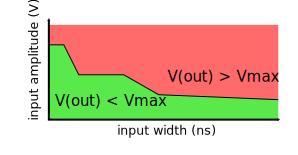
\includegraphics{src/4/figures/example_curve.pdf}
  \caption{Visual representation of powered-on block testing results}
  \label{wb_cz_curve_example}
\end{figure}

% How to improve the displayed information
Presence or absence of a failure is not the only information that can be obtained by monitoring the output.
Because soft-failures are temporary issues, their duration is also very relevant.
Using the same characterization setup as before (Fig. \ref{block_function_cz}), it is possible to also measure the duration of a failure.
It is possible to improve table \ref{simulation-results} by replacing the fail or no-fail flag by the duration of the fail.
This is illustrated in table \ref{simulation-results-bis}.
With those example values, for an input pulse stress of 5V with a input pulse width of 1ns, no failure was recorded.
On the other hand, with a 5V 1\textmu{}s stress, a failure was recorded and the output waveform crossed the threshold during 2\textmu{}s.
A 15V 1\textmu{}s stress caused a failure that lasted 30\textmu{}s.

\begin{table}[!h]
\centering
\begin{tabular}{@{}lcccc@{}}
\toprule
    & \multicolumn{1}{l}{1ns}      & \multicolumn{1}{l}{10ns}     & \multicolumn{1}{l}{100ns}    & \multicolumn{1}{l}{1us}     \\ \midrule
15V & {\color[HTML]{00D2CB} 110ns} & {\color[HTML]{FFCB2F} 150ns} & {\color[HTML]{FE0000} 30us}  & {\color[HTML]{FE0000} 30us} \\
10V & {\color[HTML]{32CB00} }      & {\color[HTML]{00D2CB} 125ns} & {\color[HTML]{F8A102} 540ns} & {\color[HTML]{FE0000} 30us} \\
5V  & {\color[HTML]{32CB00} }      & {\color[HTML]{32CB00} }      & {\color[HTML]{32CB00} }      & {\color[HTML]{F56B00} 2us}  \\
\bottomrule
\end{tabular}
\caption{Example result set containing failure width information}
\label{simulation-results-bis}
\end{table}

% How to improve the curve from the improved table
This improvement can also be transfered to the curve representation.
A gradient is used rather than a fail or no-fail area.
The gradient color for each location corresponds to the failure duration the output.
The figure \ref{wb_cz_curve_example_v2} provides an example of this improved representation.
In this figure, the warmer the gradient, the longer the output is disturbed.

\begin{figure}[!h]
  \centering
  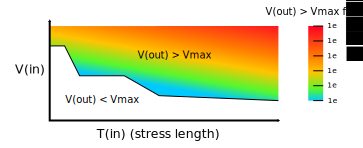
\includegraphics{src/4/figures/example_curve_v2.pdf}
  \caption{Improved curve for Wunsch and Bell powered-on characterization}
  \label{wb_cz_curve_example_v2}
\end{figure}

The gradient can also be discretized into a few aeras for better readability as shown in figure \ref{wb_cz_curve_example_v2_discrete}.
This representation looses some information compared to the gradient one but is easier to generate and read.

\begin{figure}[!h]
  \centering
  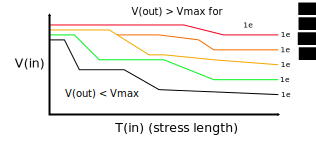
\includegraphics{src/4/figures/example_curve_v2_discrete.pdf}
  \caption{Improved discrete curve for Wunsch and Bell powered-on characterization}
  \label{wb_cz_curve_example_v2_discrete}
\end{figure}

% Summarize the method
In this section, a method was detailled to extract the robustness of a block function.
It relies on injecting pulses on an input and watching for changes on an output.
After characterization, a model can be constructed.
It is composed of a characterization table and a failure criteria.
Fig. \ref{fig:principle-transfert-func} provides a visual representation of this model.

\begin{figure}[!h]
  \centering
  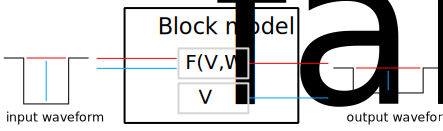
\includegraphics[width=0.8\textwidth]{src/4/figures/principle_transfert_function.pdf}
  \caption{First modelling method}
  \label{fig:principle-transfert-func}
\end{figure}

% Explain the visual representation
The model accepts a rectangular input waveform and returns a rectangular output waveform (Fig. \ref{fig:principle-transfert-func}).
More specifically, the width (red arrow) and the amplitude (blue arrow) of the input signal are the two parameters required by the model.
Those values are fed to the characterization table to calculate the width of the output signal.
The characterization table is represented by the function $F(V,W)$, with $V$ corresponding to the input amplitude and $W$ to the input width.
The failure criteria V\textsubscript{fail}, employed for establishing the characterization table, is also used directly as amplitude value for the output signal.
Using the failure criteria for modelling the output amplitude is a large approximation and validity of this approach is checked in the next section.
Ultimately, the goal is to investigate whether or not a fixed failure threshold is suitable for ESD functional analysis.

% What is done next
In the next section, those individual block models are chained together to deduce the robustness of a complete function.
The processed is explained in detailed and is later applied on a practical case.

\subsection{Block models chaining}
\label{sec:block-chaining}

% Explain the chaining mechanism
This section presents the second phase of the method that consists in chaining individual block models to deduce the robustness of a higher-level function.
To present this concept of chaining models, a purely hypothetical example is taken first.
The method is tested with a true case study afterwards.
The characterization process detailed previously is performed on two different blocks, called $A$ and $B$ (see Fig. \ref{example_toplevel_function}).
Those two blocks are part of an hypothetical higher-level function.
The function has an external input (called \textit{in}) and an external output (called \textit{out}).
A stimulus is injected on the external input and the job of the model chain is to predict what will be the approximate waveform on the external output.
Both blocks were previously (hypothetically) characterized and failure criteria V\textsubscript{fail} for block $A$ is 5 V and 2 V for block $B$.
In practice, the threshold selection is done either from the block specification or datasheet, or directly from its design.

\begin{figure}[!h]
  \centering
  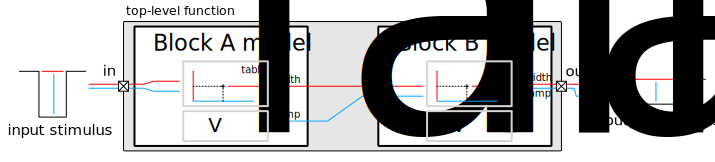
\includegraphics[width=\textwidth]{src/4/figures/example_top_level_function.pdf}
  \caption{Top-level function model constituted of 2 blocks}
  \label{example_toplevel_function}
\end{figure}

% What is the input stress
The input stimulus is a rectangular 100 ns wide pulse with a 15V amplitude.
Those two properties are fed into the hypothetical characterization of block $A$ (Fig. \ref{example_complete_curve}).
In the graph, multiple curves can be identified, each corresponding to a boundary between two disturbance durations.
For a point located below the green curve (with label "10 ns"), no stress was recorded on the output.
For a point located above the 10 ns curve and below the 100 ns curve, a stress was indeed recorded with a duration comprised between 10 ns and 100 ns.
The exact value between those two boundaries is not known with this this kind visualization.
In the analysis, the lower boundary is always chosen because the output is disturbed for at least this value.

\begin{figure}[!h]
  \centering
  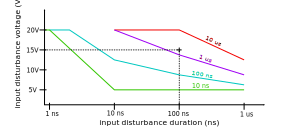
\includegraphics{src/4/figures/example_complete_curve.pdf}
  \caption{Model A curve and determination of impact of the TLP pulse - values in color represent the duration of failure on the output}
  \label{example_complete_curve}
\end{figure}

% Interpretate stress to deduce net1
With the given 15 V 100 ns stimulus, the curve predicts that the output will fall below 5 V (V\textsubscript{fail} of block A) during 1 \textmugreek{}s.
Those two values describe the signal on the output of block A.
Those values are now used to describe the stimulus on block B, since both blocks are connected.
The failure criteria that was used to extract the characterization curve also serves as amplitude for the output signal.
It means that with a 5V failure criteria, if a failure is recorded, the output waveform is approximated to also have an amplitude of 5V.

% Use net1 as input of next block
Fig. \ref{example_complete_curve_B} shows an example curve for model B.
The location of the stimulus from block A (5 V and 1 \textmugreek{}s) is also placed on the curve.
The curve predicts that with this stimulus, block B will be disturbed during 10 \textmugreek{}s with an amplitude of 2 V (V\textsubscript{fail} of block B).

\begin{figure}[!h]
  \centering
  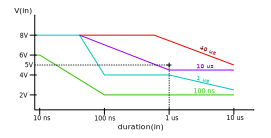
\includegraphics{src/4/figures/example_complete_curve_B.pdf}
  \caption{Model B curve and determination of impact of the TLP pulse}
  \label{example_complete_curve_B}
\end{figure}

% Repeatable process
This process can be repeated in theory with as many blocks as required by the original design, until the final pin is reached.

\subsection{Application to the test vehicle}

The method described in both previous sections (\ref{sec:block-failure-cz} and \ref{sec:block-chaining}) is tested in simulation on real blocks.
More precisely, it will be tested against the regulation function of the testchip.

% Which pins are selected for characterization
This function is composed of three blocks, a pre-regulator, a bandgap and a regulator.
For each one, an input and output pin are selected.
The input/outputs that play a key role on the regulation function were selected on the regulation function.
Details of the selected pins is given in Table \ref{selected-pins-for-cz}.

%TODO: To simplify
\begin{table}[]
\centering
\begin{tabularx}{\linewidth}@{}|c|c|c|c|c|c|c|@{}}
\toprule
{ \textbf{IC block}} & { \textbf{input pin}}                 & \multicolumn{1}{l|}{{ }} & { }                                & \multicolumn{1}{l|}{{ }}               & { \textbf{output pin}}            & { }                          \\ \midrule
{ }                  & { \textbf{specification}}             & { \textbf{DC value (V)}} & { \textbf{stress amplitude range}} & { \textbf{stress width range}}         & { \textbf{specification}}         & { \textbf{Failure criteria}} \\ \midrule
{ pre-regulator}     & { external supply battery connection} & { 12V}                   & { -1V to -10V with 1V step}        & { 1ns to 1000ns with 30 pts log scale} & { 9V clamped voltage}             & { vclamp9 \textless 0V}      \\ \midrule
{ bandgap}           & { 9V clamped voltage}                 & { 9V}                    & { -1V to -15V with 1V step}        & { 1ns to 1000ns with 30 pts log scale} & { bandgap voltage 2.5V reference} & { vref2p5 \textless 1.25V}   \\ \midrule
{ regulator}         & { bandgap 2.5V reference}             & { 2.5V}                  & { -0.5 to -10V with 0.5V step}     & { 1ns to 1000ns with 30 pts log scale} & { regulated 2.5V 20mA capability} & { v2p5 \textless 2.1 V}      \\ \bottomrule
\end{tabularx}
\caption{Selected pins for characterization and characterization limits}
\label{selected-pins-for-cz}
\end{table}

% Talk about the characterization limits
The characterization is done using negative voltages.
The goal is to exploit the weakness of the testchip against negative pulses discovered and highlighted in section \ref{sec:testchip_study}.
Basically, it was observed for sufficiently high negative voltage a short pulse can cause a full restart of the system.
The time taken by this restart, observed on the regulator output, is several order of magnitudes longer than the original pulse injected on the pre-regulator input.

% failure criteria chosen
The failure criteria for the pre-regulator is a voltage lower than 0V on the output.
It corresponds to a situation worse than the unpowered state, where all nets are at 0V.
The failure criteria for the bandgap is a voltage lower than 1.25V on the 2.5V reference output.
Finally, the failure criteria for the regulator, which is also the failure criteria for the complete function, is a voltage lower than 2.1V on the 2.5V regulated output.
This criteria corresponds to a voltage below which digital cells using this supply will fail to function properly.

% Which load value for characterization
The test setup described in section \ref{sec:block-failure-cz} requires a characterization load to simulate the impact of neighbor blocks.
In a first time, a very simplistic model is employed for this load.
An arbitrary load value of 1M\textgreek{Omega}\ is initially chosen, just to perform a preliminary test.
The impact of this load on the characterization will be evaluated later on in the analysis.

% Simulation process
For each block, the characterization testbench is setup and a set of simulations is ran.
This set is calculated with the characterization range given in Table \ref{selected-pins-for-cz}.
This type of parameterized simulations can be efficiently distributed on multiple machines.
This way, the complete characterization of a block does not take longer than the time taken by a single simulation.
Once all simulations are run, the results are analysed and plotted using the method detailed in the previous sections.

% Talk about the output
These characterization curves are given in Figs. \ref{pre_regu_wb}, \ref{bandgap_wb} and \ref{regu_wb}.
The characterization of the pre-regulator (fig. \ref{pre_regu_wb}) is plotted using the stress amplitude only on the X axis.
The stress amplitude is the pulse voltage set in the pulse generator SPICE model.
On the other hand, the bandgap and regulator curves are using instead the voltage probed on the input net during the stress.


% TODO: Why curve 1 has different x-axis
The reason for using the set voltage directly, and not

\begin{figure}[!htbp]
  \centering
  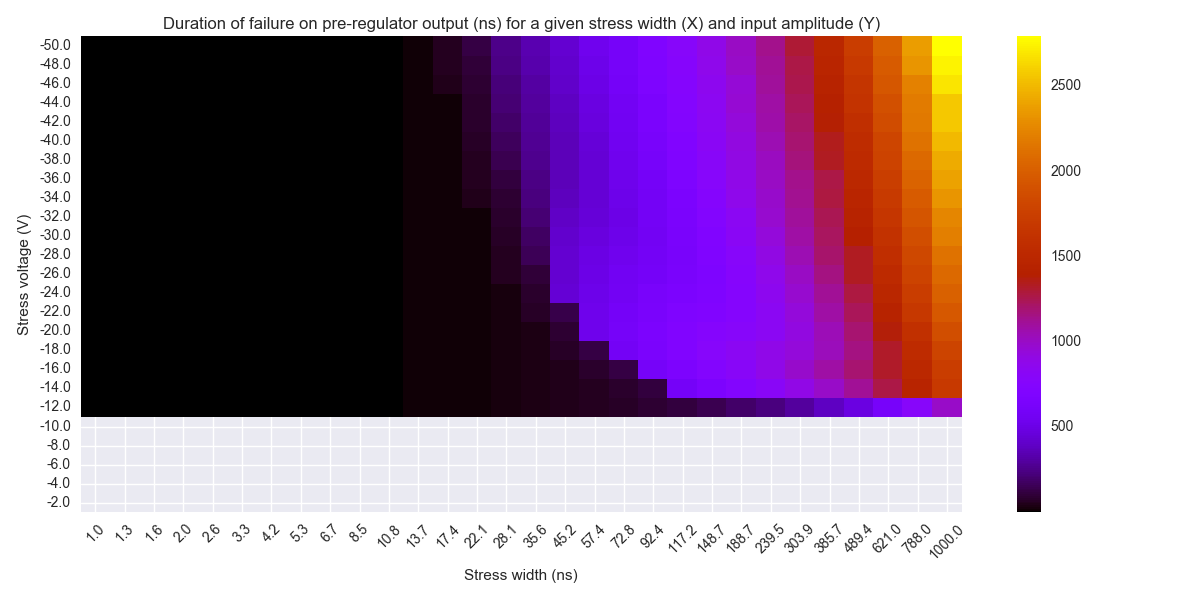
\includegraphics[width=\textwidth]{src/4/figures/preregulator_cz.png}
  \caption{Pre-regulator 9V clamped-output characterization}
  \label{pre_regu_wb}
\end{figure}

\begin{figure}[!htbp]
  \centering
  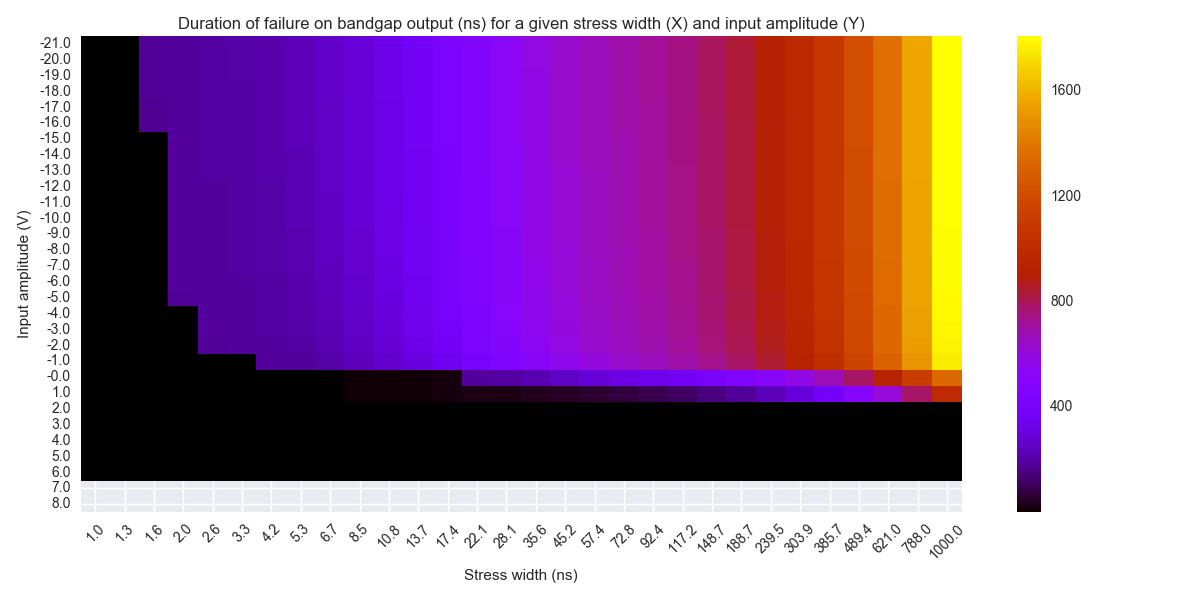
\includegraphics[width=\textwidth]{src/4/figures/bandgap_cz.png}
  \caption{Bandgap 1.0V reference characterization}
  \label{bandgap_wb}
\end{figure}

\begin{figure}[!htbp]
  \centering
  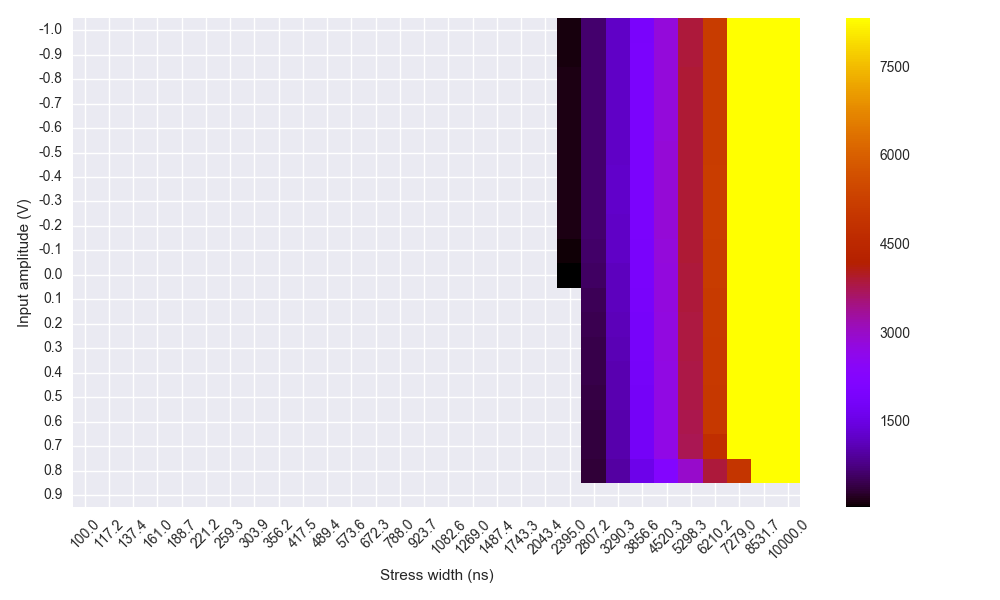
\includegraphics[width=\textwidth]{src/4/figures/regulator_cz.png}
  \caption{Regulator 2.5V supply characterization}
  \label{regu_wb}
\end{figure}

% Characterization done, now perform chaining
After the characterization phase, it is now possible to chain the models together.
The goal is to evaluate the entire function's robustness with the method described in \label{sec:block-chaining}.
A rectangular pulse is injected on the global input (pre-regulator input).
The chain of models is used to predict, without running any more simulations, the failure or not on the output pin.
For the purpose of this test, the input stress will be generated by a \gls{tlp} generator, producing a pulse of 100ns duration and -30V amplitude.

% Do it on one pulse config
%TODO: Review values
First, the coordinaates (100ns, -30V) are reported on curve \ref{pre_regu_wb}, the first block model of the system.
This point indicates a failure on the output of the pre-regulator, for a duration of 500ns.
The failure criteria is 0V on the output.
This gives the next point coordinates (500 ns, 0V).
This point is reported on the bandgap's model, the next block in the system.
Using these coordinates in the curve \ref{bandgap_wb} indicates a failure on the bandgap output for about 800ns.
Since the failure criteria for the bandgap is 0V on the output, the next point coordinates are (800ns, 0V).
They are used as an input on the final block's model (fig. \ref{regu_wb}).
Reporting those coordinates, no failure is expected on the regulator output.

In conclusion, the model chain estimated that for a -30V 100ns stress on the input, the regulation function will not be at fault (output < 2.1V).

% Same analysis but with a TLP stress that will cause a fail
The same analysis is done for a -30V stress but with a longer width of 1us.
The failure on the pre-regulator is then estimated to last 2300 ns.
In turn, the bandgap is estimated to fail during 3000 ns.
Finally, the output of the regulator and thus the entire function is estimated to fail during 1500ns.

% Perform standard complete simulation for reference
Those results are then tested against a complete simulation of the entire regulation function (all three block).
The simulation circuit is given Fig. \ref{fig:reference_simu_circuit}.
This simulation uses transistor-level block models.
It will serve as a reference to compare the model-chain against it.

% How will the simulation be conducted
For this simulation, the same input stress are used than previously, and the global output is monitored for failures.
To check the validity of the models at each stage, intermediate voltages are also monitored, at the output of the pre-regulator and the bandgap.
The simulation of the input, pre-regulator output, bandgap output and final (regulator) output are given fig. \ref{fig:reference_simu}.

\begin{figure}[!htbp]
  \centering
  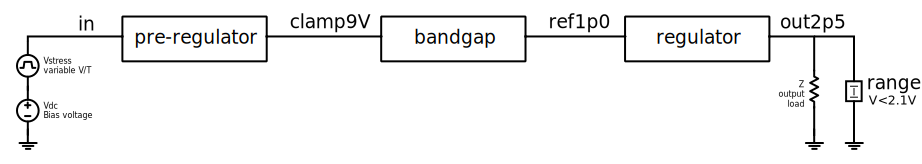
\includegraphics[width=\textwidth]{src/4/figures/complete_simulation_setup.pdf}
  \caption{Complete reference simulation circuit}
  \label{fig:reference_simu_circuit}
\end{figure}

%TODO: Zoom on the area of interest
\begin{figure}[!htbp]
  \centering
  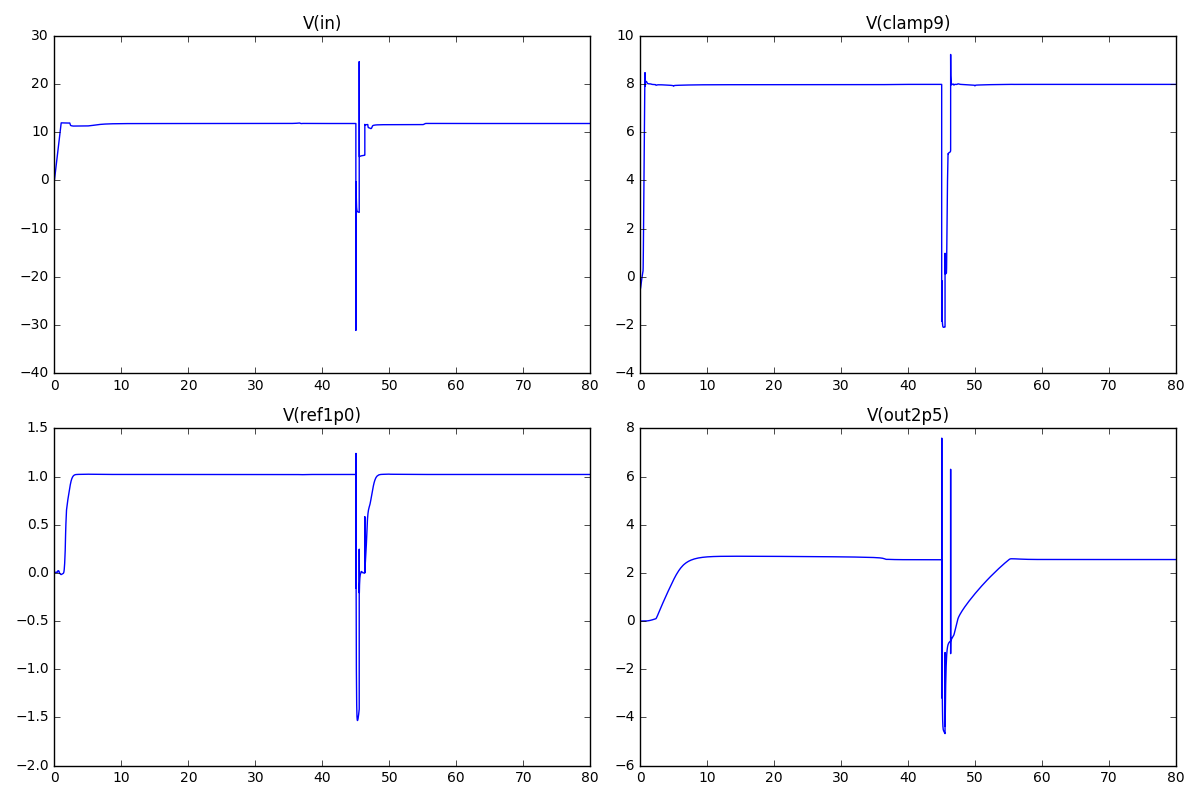
\includegraphics[width=\textwidth]{src/4/figures/total_simulation.png}
  \caption{Reference simulation waveforms}
  \label{fig:reference_simu}
\end{figure}

% Result of the simulation
The simulation showed that for the given stress, the output V(out2p5) will go below 2.1V for 8160ns.
%TODO: Make the comparison with chain models
There is a rather large difference with the model chain.
To try to explain this difference, intermediates nodes are monitored.

% Error at the first block
The output of the pre-regulator is below X V (failure criteria) for XX ns in the full simulation while the model predicted XX ns.
Already, at this first block, there is a large difference between the simulation and the model.

% Error at the second block
The output of the bandgap (second block) shows even a higher difference.
In simulation, the output goes below XX V for XXX ns, while the model predicted XXX ns.

% Conclusion regarding this first simulation
Not only each curve introduces an important error, but errors tend to accumulate after each block.

% Test further simulation vs model
To test further the model versus the reference simulation, a set of different stresses are injected, with different properties.
The goal is to test the model on a larger set of input stresses.
For each stress, the result predicted by the model and the result obtained by the reference simulation are compared.
Results are summarized in table \ref{tab:comparison-multiple-pulses}.
The entire process is summarized in fig. X.

\begin{table}[!htbp]
\centering
\begin{tabular}{@{}|c|c|c|c|@{}}
\toprule
\multicolumn{2}{|c|}{\begin{tabular}[c]{@{}c@{}}Stress\\ properties\end{tabular}} & \multicolumn{2}{c|}{Results} \\ \midrule
duration (ns)                           & amplitude (V)                           & Reference      & Model       \\ \midrule
1 ns                                    & -5V                                     & no fail        & no fail     \\ \midrule
1 ns                                    & -10V                                    &                &             \\ \midrule
1 ns                                    & -15V                                    &                &             \\ \midrule
10 ns                                   & -5V                                     & fail 10ns      &             \\ \midrule
10 ns                                   & -10V                                    &                &             \\ \midrule
10 ns                                   & -15V                                    &                &             \\ \midrule
50 ns                                   & -5V                                     &                &             \\ \midrule
50 ns                                   & -10V                                    &                &             \\ \midrule
50 ns                                   & -15V                                    &                &             \\ \midrule
500 ns                                  & -5V                                     &                &             \\ \midrule
500 ns                                  & -10V                                    &                &             \\ \midrule
500 ns                                  & -15V                                    &                &             \\ \bottomrule
\end{tabular}
\caption{Comparison between simulation and reference for several pulse configurations}
\label{tab:comparison-multiple-pulses}
\end{table}

% Conclusion regarding the tables, differences observed

%TODO Review next
% Where does error come from ? Load impedance
Previously, it was indicated that all WnB curves were extracted with a fixed Zout = 1M\textOmega.
When connected together, each block (pre-regulator, bandgap, regulator) sees a load impedance on its output much different than that.
Thus, it is important to evaluate the impact of this value on the Wunsch and Bell characterization curve.
The pre-regulator is characterized again, this time with a load impedance of 100\textOmega.
This value is rather small impedance, but sufficiently high to not draw too much current on the pre-regulator.
This second characterization is given fig. X.

%TODO: CHARACTERIZATION WITH Z LOW IMPEDANCE

This characterization is compared with the one extracted with 1M\textOmega\.
To make the comparison easier, curves for failure above 1ns, 10ns, 100 ns and 1us were plotted separately (see fig. X).
MAKE COMPARISON

%TODO: COMPARISON Z LOW IMPEDANCE Z HIGH IMPEDANCE 2 * 2 1n -> 1u

SO FAR, CONSIDERED IMPEDANCE AS STATIC AND REAL.
TALK ABOUT IMAGINARY IMPEDANCES, AND DYNAMIC IMPEDANCES

TALK ABOUT ERROR CAUSED BY GRADIENT ?


\subsection{Conclusion regarding bottom-up block failure modeling method}

On paper, this method was rather promising in terms of applicability.
A block could be characterized once, and reused in different places.
The robustness of a full system could have been quickly and easily deduced from the models of its parts.

However, with the study case exposed earlier, several issues arose that clearly limit the ability of the model to perform as expected.

The main issue with this modelling method is the fact that it relies too much
on the value of the output load for performing the characterization of a block.
This load depends on many different parameters.
And this value will change in function out the block connected on the output (think about block-reuse)
Also, this value may not be constant in frequency.
And this value may also not be constant in time (multiple operating modes, biasing points, etc).

% SHOW SIMULATIONS FOR THIS PROBLEM OF IMPEDANCE VARIATION

% DIRECTIVITY - WE ASSUME STRESS AND FAILURES PROPAGATE FROM INPUT TO OUTPUT. MAY NOT BE THE CASE. ALSO, MAY NOT WORK IN REVERSE WITH SINGLE2MANY BLOCK CONNECTIONS

Another issue, this method is limited to a binary FAIL/NO FAIL criteria.
Not only this criteria is arbitrary (in some cases, the specification could be used to set it), but
for most purely-analog blocks, there will not be a clear failure, rather, most
nets will have degraded values until maybe biasing of the block completely fails.
In this case, the binary criteria hides a lot of information about the degradation.

ANY CLUES TO OVERCOME THESE ISSUES ?

ALSO, FAILURE MAY NOT PROPAGATE IN THIS ONLY WAY, BUT BACKWARD TOO

The main reason why this approach was investigated was for its very interesting modularity
that was highly suitable for block reuse workflow.

However, because of the intrisic interactions between block functions in an integrated circuit,
TRY TO EXPRESS BETTER WHAT PRINCIPLE OF THIS METHOD BOUNDS IT TO FAIL

this approach seems to be bound to fail for building a reusable model for an IC block that could predict
ESD failures at the architecture level and during the IC architecture phase.
